\section{Introduction}
\label{sec:intro}
The Gemma 4 Developer Agent competition~\citep{Markowitz2026GoogleGemma} asks for a Gemma 4~\citep{Team2026Gemma4} agent that fixes real bugs on consumer hardware. The standard route to a better agent is post-training. A LoRA adapter from our own small reinforcement-learning (RL) pipeline solved 32, 30 and 36 of our 170 development tasks in three batches. In those batches the unedited model solved 28, 24 and 22. These batches did not serve the adapter alongside the unedited model. In two of them the adapter also led an always-on edit of this paper (30 and 36 against 28 and 32), again not served together. No gated edit ran beside the adapter (\S\ref{sec:discussion}).

A second route appeared this month. \citet{Takehi2026SparksWeightspace} showed that a frontier LLM can read and write the weights of a small model without gradients. They named the approach weight-space programming. \citet{Bennington2026GradientfreeWeight} compiled activation-derived directions into the MLP down-projections of Qwen3.8-27B and tested them against a norm-matched random control. Both evaluate their edits on single-turn benchmarks. An agent is a harder target. An episode is a sequence of up to 34 tool calls (about 10 on average for the unedited model). The edit must change a decision that recurs across the episode, and the outcome (hidden tests pass) depends on every decision in it. Measurement is also harder: with greedy decoding, the unedited model solved between 21 and 30 of the same 170 tasks across 21 complete runs.

\begin{figure}[t]
\begin{center}
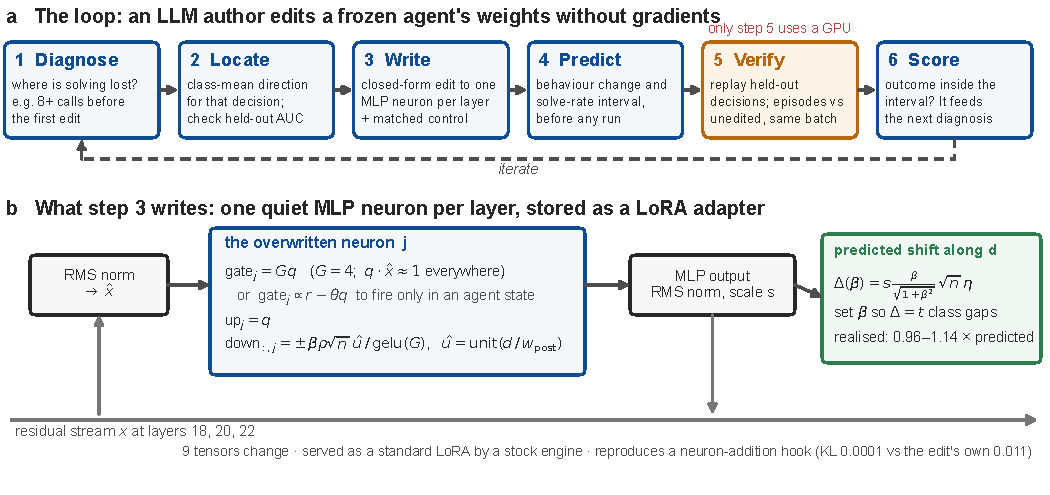
\includegraphics[width=1.0\linewidth]{figures/fig1_loop.pdf}
\end{center}
\caption{\textbf{The method.} (a) The loop of this paper. An LLM author diagnoses a failure from logged episodes of a frozen Gemma 4 E4B coding agent and locates a direction for the decision involved. It writes a closed-form edit and a matched random control and writes down its prediction. It verifies the edit against the unedited model in the same batch and scores the prediction. No step computes a gradient; only verification uses a GPU. (b) The edit of step 3. In each of three layers, the quietest MLP neuron is overwritten. The new neuron fires at a constant level (or only in a chosen agent state) and writes along the direction $d$. Eq.~(\ref{eq:shift}) predicts the shift, and the build measures it.}
\label{fig:loop}
\end{figure}

This paper delivers cheap, precise, verifiable control of a coding agent's decisions by LLM-written weight edits, and a measured account of when such control does and does not raise solve rate. We credit the idea of LLM-written weights to the two works above. Four things differ here. First, the target is a decision of a multi-step agent, not a single-turn output. Second, edits are gated on agent state instead of adding a constant direction; for example, one gate fires before the episode's first edit, with measured leakage elsewhere (\S\ref{sec:control}). Third, each edit carries a written prediction that we score afterwards. Fourth, we compare three LLM authors under one brief. We ask three questions. Does an edit move a named decision where a matched random control does not? Does it raise the solve rate beyond its control? How often is the author's written prediction right?

\noindent Contributions, in order of the paper:
\begin{itemize}
    \item \textbf{Method} (\S\ref{sec:method}): to our knowledge the first LLM-authored weight edits for a multi-step coding agent, gated on agent state, sized in closed form and packed exactly into a LoRA~\citep{Hu2021LoraLowrank} adapter that a stock engine serves.
    \item \textbf{Decision control} (\S\ref{sec:control}): always-on edits move three decisions with a dose-response on held-out decisions, while matched random controls stay near the unedited value.
    \item \textbf{Solve rate} (\S\ref{sec:devgain}--\ref{sec:heldout}): the best edit solved 30.3 against 25.3 tasks ($p = 0.014$ uncorrected); it does not survive Holm correction, and the pre-registered held-out test agreed in sign ($+3.0$, $p = 0.50$).
    \item \textbf{Diagnosis and evaluation lessons} (\S\ref{sec:diagnosis}, \S\ref{sec:negative}, \S\ref{sec:discussion}): a small coding agent fails by inconsistency, not incapacity, and solve rate is governed by run-to-run variance and selection.
    \item \textbf{Three-author benchmark} (\S\ref{sec:arena}): twelve edits and three controls from Claude, GPT and Gemini, each with a written 80\% interval scored afterwards.
\end{itemize}
We release the edit builder, an episode and decision dataset with labelled activations, and the three authors' prediction files as a reusable resource, together with all edits, pre-registrations and per-task results.

